% Template: parabol y = a x^2 trên hệ trục Oxy.
% Đổi \a để có hệ số khác. Đổi \xmin, \xmax để mở rộng khoảng vẽ.
\documentclass[border=5pt]{standalone}
\usepackage{tikz}
\usepackage{pgfplots}
\pgfplotsset{compat=1.18}
\begin{document}
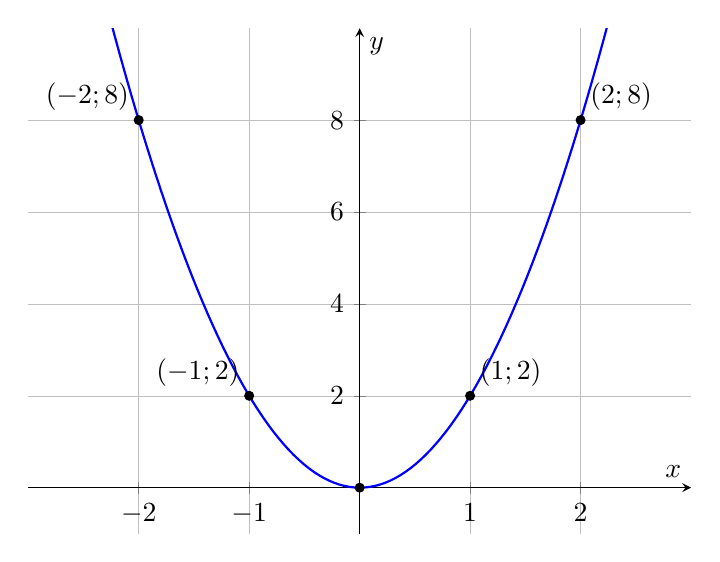
\begin{tikzpicture}
  \begin{axis}[
      axis lines=middle,
      xlabel=$x$, ylabel=$y$,
      xmin=-3, xmax=3,
      ymin=-1, ymax=10,
      xtick={-2,-1,0,1,2},
      ytick={2,4,6,8},
      grid=both,
      grid style={line width=.1pt, draw=gray!30},
      major grid style={line width=.2pt,draw=gray!50},
      width=10cm, height=8cm,
      samples=101,
      domain=-2.3:2.3,
    ]
    % a = 2 -> y = 2x^2
    \addplot[blue, thick]{2*x^2};
    % Đánh dấu vài điểm trên parabol
    \addplot[only marks, mark=*, mark size=1.6pt]
      coordinates {(-2,8) (-1,2) (0,0) (1,2) (2,8)};
    % Nhãn cho điểm
    \node[above left] at (axis cs:-2,8) {$(-2;8)$};
    \node[above left] at (axis cs:-1,2) {$(-1;2)$};
    \node[above right] at (axis cs:1,2) {$(1;2)$};
    \node[above right] at (axis cs:2,8) {$(2;8)$};
  \end{axis}
\end{tikzpicture}
\end{document}
